\chapter{The Divided Line of Action}

\epigraph{``The sun is the offspring of the Good, which the Good begot as its
analogue.''}{\textcite{plato1997complete}, \emph{Republic} 508b}

\section{The Sun and the Good}

In the \emph{Republic}, Socrates describes the Form of the Good as the source
of all intelligibility --- the sun of the intelligible realm. Just as the visible
sun illuminates physical objects and enables the eye to see them, the Form of
the Good illuminates the Forms and enables the mind to know them. The Good is
not itself seen; it is the condition for all seeing.

Our \physis\ is the analogue of the Good. It is not itself an action but the
condition for all right action. It is the source of the intelligibility of
action --- the standard by which an act is judged to be coherent or incoherent,
effective or inert, aligned or misaligned. The practitioner does not see \physis\
directly; they see the coherence of their actions, which is \physis\ reflected
in the world.

\section{The Divided Line}

Socrates divides the intelligible realm into four segments, arranged by
increasing clarity \parencite[VI.509d--511e]{plato1997complete}:

\begin{figure}[ht]
\centering
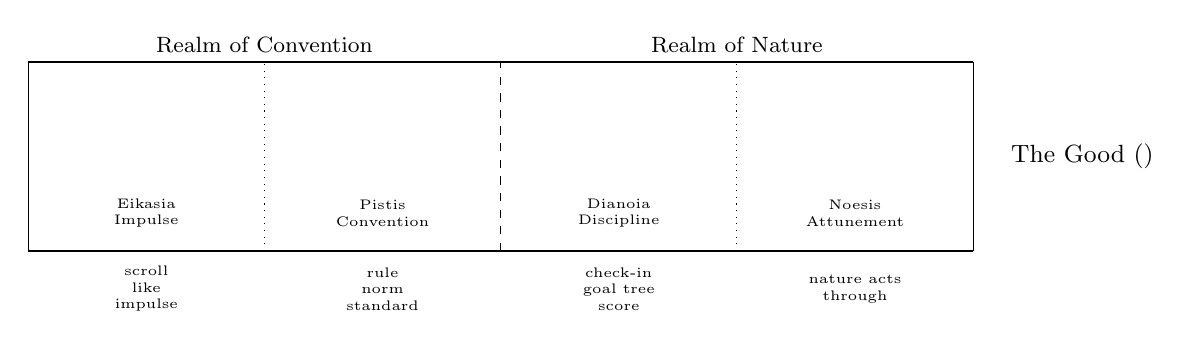
\begin{tikzpicture}[scale=1.2]
  \draw (0,0) -- (10,0);
  \draw (0,2) -- (10,2);
  \draw (0,0) -- (0,2);
  \draw (10,0) -- (10,2);

  \node[anchor=west, font=\small] at (10.3,1) {The Good (\physis)};

  \draw[dashed] (5,0) -- (5,2);
  \node[anchor=south, font=\footnotesize] at (2.5,2) {Realm of Convention};
  \node[anchor=south, font=\footnotesize] at (7.5,2) {Realm of Nature};

  \draw[dotted] (2.5,0) -- (2.5,2);
  \draw[dotted] (7.5,0) -- (7.5,2);

  \node[font=\tiny, align=center] at (1.25,0.4) {Eikasia\\Impulse};
  \node[font=\tiny, align=center] at (3.75,0.4) {Pistis\\Convention};
  \node[font=\tiny, align=center] at (6.25,0.4) {Dianoia\\Discipline};
  \node[font=\tiny, align=center] at (8.75,0.4) {Noesis\\Attunement};

  \node[font=\tiny, align=center, text width=18mm] at (1.25,-0.4) {scroll\\like\\impulse};
  \node[font=\tiny, align=center, text width=18mm] at (3.75,-0.4) {rule\\norm\\standard};
  \node[font=\tiny, align=center, text width=18mm] at (6.25,-0.4) {check-in\\goal tree\\score};
  \node[font=\tiny, align=center, text width=18mm] at (8.75,-0.4) {nature acts\\through};
\end{tikzpicture}
\caption{The divided line of action: each level corresponds to a mode of acting, from
unreflective impulse to nature-aligned attunement.\label{fig:dline}}
\end{figure}

We extend the line to action. At each level, the practitioner acts in a
different mode, with a different kind of knowledge of what they are doing.

\subsection{Eikasia: The Arbitrary Act}

The lowest segment is the act without reflection --- impulse, habit, social
conformity. The practitioner at this level acts because ``that's what one does,''
or because the impulse arose, or because the algorithm recommended it. They have
no account of why they act; their action is a shadow of a shadow, a reaction to
a stimulus whose origin they do not know.

This is the default state of action in the age of technology. The attention
economy is designed to produce this kind of action: the scroll, the like, the
click --- all eikastic, all without reflection, all shadows of intentions that
are not the practitioner's own.

\subsection{Pistis: The Conventional Act}

The second segment is action governed by convention --- the rule, the social
norm, the professional standard. The practitioner at this level acts because
there is a rule that says to act this way. They have an account of their action,
but it is borrowed from the group. ``We do it this way because this is how it
has always been done.''

This is better than eikasia, but it is not yet governed by nature. Convention
(\emph{nomos}) is a human artefact; it may align with nature or not. Most
conventions are sedimented from past discoveries about what works, but they
have become detached from the natural grounds of their authority. The
practitioner follows the rule without knowing why the rule exists.

\subsection{Dianoia: The Nature-Aligned Act}

The third segment is action governed by inquiry into nature. The practitioner
at this level does not follow rules but \emph{discovers} principles. They act
according to the disciplines described in Book III: they check in, they seek
witness, they stake their skin, they maintain their rhythm, they review their
patterns. They have an account of their action that is their own, grounded in
their observation of what works.

The \praxis\ platform supports this level of action. The goal tree is a
hypothesis about what the practitioner's nature requires; the check-in is the
experimental record; the coherence score is the result. The practitioner at
this level is a scientist of their own action.

\subsection{Noesis: Action as Nature's Self-Expression}

The highest segment is action that has become indistinguishable from nature's
own movement. The practitioner no longer acts ``according to'' nature; they act
\textit{as} nature. Their action is not a choice they make but a recognition of
what must be done. They have ascended beyond the disciplines to a state of
spontaneous right action.

This is the practitioner-king of Book V. They do not need the \praxis\ platform,
for the platform has served its purpose as training wheels. But they may choose
to remain on the platform as a witness for others --- the one who, having seen
the sun, returns to the cave.

\section{The Sun of Action}

What illuminates this entire line? Not a rule, not a principle, not a command
--- but \physis\ itself. Nature is the sun of action, the source of the
intelligibility of every act. The practitioner can only see the coherence of
their action because nature provides the light by which coherence is visible.

The \physis\ engine does not create this light; it \emph{channels} it. The
embedding space, the semiotic grid, the coherence scale, the dream function ---
these are not inventions but discoveries. They are the structure of nature
itself, made computationally tractable. The engine is the technical form of a
philosophical truth: nature is the governor of action because nature is the
source of the intelligibility of action.

\section{Escaping the Cave of Convention}

The divided line of action reveals that the escape from convention (nomos) to
nature (physis) is not a single leap but a graded ascent. The practitioner does
not go from blindness to sight in one step but through four stages of increasing
clarity. Each stage has its own form of action, its own relation to knowledge,
its own mode of coherence.

The \praxis\ platform and the \physis\ engine together provide the infrastructure
for this ascent. The platform structures the intermediate stages; the engine
provides the measure of progress. But the ascent itself is the practitioner's
own work --- the work of bringing their action from the darkness of impulse
into the light of nature.
